\section{はじめに}

床に引いた黒い線を追う差動二輪型のライントレースロボットを観察する。望ましい動きは、線の中央を一定の速さで進むことである。しかし実際の軌跡は左右にふれ、曲がり始めで外側へ膨らみ、左右の車輪の回転量も同じにはならない。開始からの経過時刻、左右のラインセンサの読み、車輪エンコーダのパルス数、線中心からの横ずれを同じ時刻に対応させると、望む経路と実際の経路の差が数値と曲線として現れる。この測った差を次の入力へ反映する仕組みを作ることが、本書の出発点である。

\begin{figure}[tb]
  \centering
  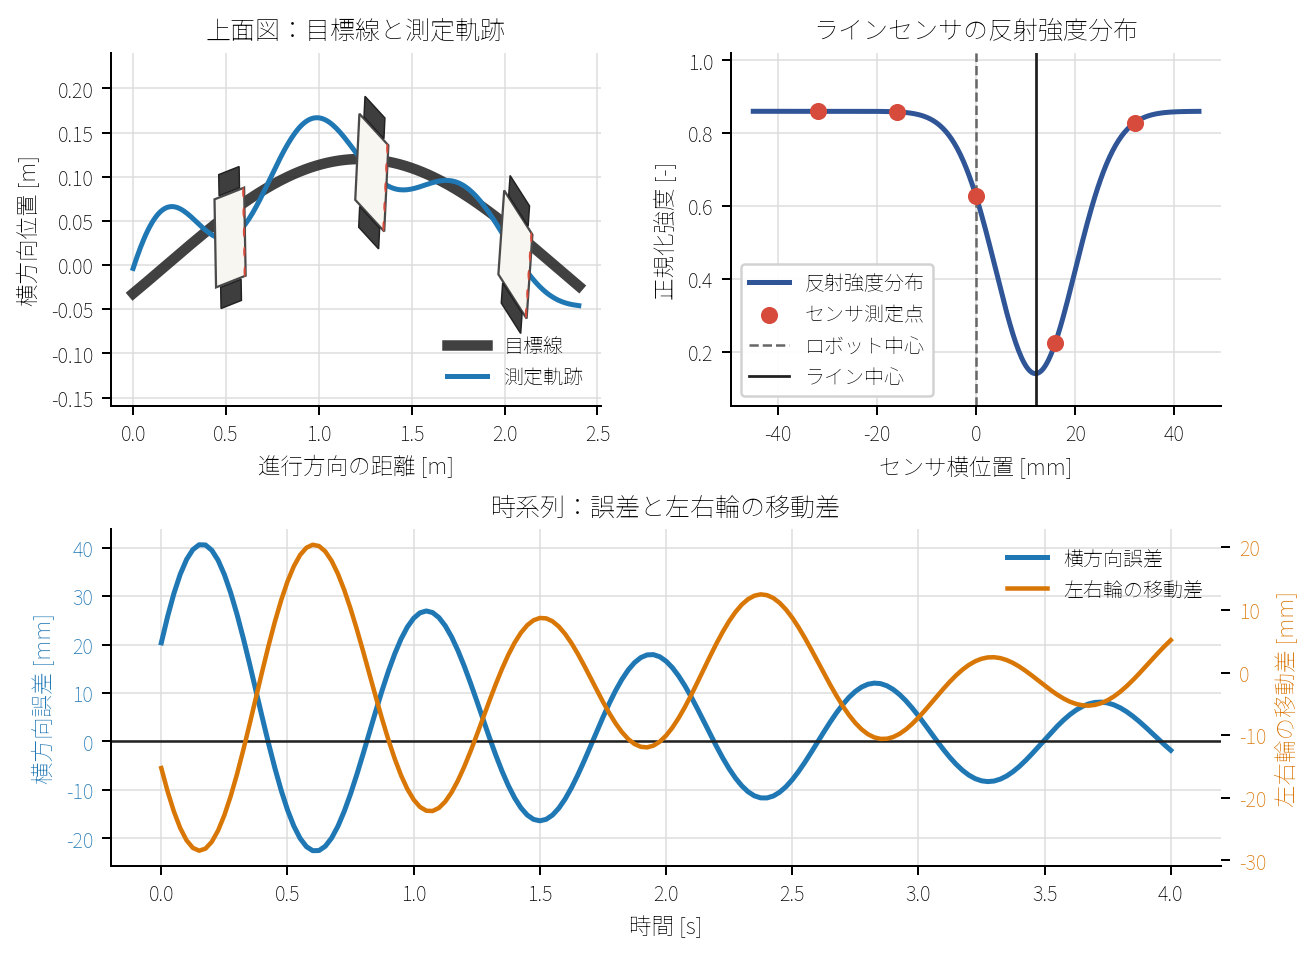
\includegraphics[width=0.96\linewidth]{figures/opening_measurement_examples.png}
  \caption{ライントレースロボットの観察から得られる最初の測定例。左上は床上の目標線と測定された走行軌跡のずれ、右上は横一列のラインセンサが線中心の偏りを強度分布として読む様子、下段は横方向誤差と左右輪の移動差の時間履歴を示す。}
  \label{fig:opening-measurement-examples}
\end{figure}

図\ref{fig:opening-measurement-examples}では、目標線そのものは床に固定されているが、測定されたロボットの中心はその線のまわりを振動している。ラインセンサの強度分布は、黒線がセンサ列の中央からどちらへずれているかを示し、左右輪の移動差はロボットが向きを変えた区間を時系列として残す。したがって、制御工学の議論は「ロボットを動かす」ことからではなく、目標値、測定値、誤差、入力の変化を同じ時間軸と単位で比べることから始まる。

本書は、中学生から大学院生までの読者が、制御工学を段階的に理解するための教科書である。初学者には、時間とともに変化する量を観察し、測定し、グラフとして読み取るところから始める。既習の数学を広く前提とするのではなく、比例関係、変化率、方程式、ベクトル、行列、確率などを、それらが制御の説明に必要となる箇所で導入する。

制御工学では、望ましい挙動と実際の挙動の差を測定し、その差を小さくする入力を設計する。したがって、対象の性質、測定できる量、加えられる入力、外乱、許容誤差を明確にする必要がある。本書では、これらの要素を時間応答、周波数応答、状態空間表現、最適化、推定、実装の順に結び付け、古典制御から現代制御までを一貫した設計理論として扱う。

各章では、先に記号や定義を一覧するのではなく、設計上の必要から概念を導入する。仮定を明示し、式の導出を追い、図やグラフによる確認を加え、主要なパラメータを変えたときの応答を比較する。この構成により、数学的な表現、物理的な解釈、設計上の判断を対応させながら、制御工学の基礎から発展的な内容までを体系的に学ぶ。
